\section{Built a mechanism that reduces the size of queries}\label{section:applied-methods:query-reduction-mechanism}

This section describes how queries can be reduced.

Apart from sharing a single cache instance, performance can be improved even further when using GraphQL within a shared caching architecture by removing fields from a query that are already in the cache. No GraphQL client for the frontend provides such a functionality out of the box. Caching in Apollo Client works with the name of the query and the parameters of the query. For example, if a query is executed against the GraphQL API, the results of the query are cached. If the same query is executed again with the same parameters, the results are fetched from the cache, if the two queries are fetching the same fields. If one query wants to fetch a field, that is not already inside the cache, the complete query is sent to the backend. Only if all fields are identical, does the query result in fetching the data only from the cache Consequently, identical queries that fetch different fields are always fetched from the server.

\bigskip

\noindent Consider listing \ref{code:applied-methods:query-all-users-reduction}, where the left query fetches all users, and the right query fetches a user by id. Both queries fetch the same data with the same fields. Both queries are sent to the GraphQL API. The second query could be omitted if the user with the given id is fetched from the cache. 

\ifshowListings
\begin{listing}[H]
\begin{minted}{typescript}
query allUsers {                        query User(id: ID!) {
  allUsers {                              User(id: id) {
    id                                      id
    username                                username
    email                                   email
    firstName                               firstName
    secondName                              secondName
  }                                       }
}                                      }
\end{minted}
\caption{Query all users for the list-view.}\label{code:applied-methods:query-all-users-reduction}
\end{listing}
\fi


For this case the Apollo Client offers cache redirects, but the redirect works only if the list- and detail-view try to fetch the exact same fields. For example if the user micro-frontend query a list of users seen in listing \ref{code:applied-methods:query-all-users-reduction} and when a user is selected, the detail-view might display the individual user like in listing \ref{code:applied-methods:query-single-user}.

In this case it is known that the user-data is already inside the cache, but fetched by a different query. The Apollo client doesn't know that and therefore tries to fetch the User from the server. But with Type-Policies can be used to tell the Apollo client where to look for the cached User. How to write such a redirect is shown in listing \ref{code:applied-methods:user-cache-redirect}.

\ifshowListings
\begin{listing}[H]
\begin{minted}{typescript}
const client = new ApolloClient({
   cache: new InMemoryCache({
     typePolicies: {
       Query: {
         fields: {
           User(_, { args, toReference }) {
             return toReference({
               __typename: 'User',
               id: args.id,
             });
           }
         }
       }
     }
   })
 });
\end{minted}
\caption{Writing a cache-redirect for the User-type}\label{code:applied-methods:user-cache-redirect}
\end{listing}
\fi

That a detail-view and a list-view are identical is very rare in applications. Therefore this approach can't be used to reduce the size of network-requests effectively. And the approach is very verbose, because this redirect has to be written for every object type.

Many feature requests in the Apollo repository call for such a feature. While browsing GitHub, I found a project that provides drop-in replacements for Apollo's GraphQL query methods. And it provides the functionality to remove fields from a query that are already in the cache. However, the big problem was that the project was developed specifically for React and the dependencies were outdated. As a result, I couldn't install it and use it within the micro frontend written in React.

The next step was to rewrite the library in TypeScript and update the dependencies. While rewriting the library, some new features were added to still be able to exploit the cache-layer.

But the library lacked the feature of cache-redirects. Therefore, the fields which were already queried by a list-view, couldn't be reduced when the detail-view was queries. I enhanced the implementation by adding a parameter, where a reference to an existing cache-object can be specified. If no reference is found in the cache, these reference to a cache-object is used to reduce the query.

In contrast to the original implementation, the new implementation is technology agnostic and can be used with every frontend framework that supports the Apollo client. For ease of use, I wrote adapters for React and Angular that have the same API as Apollo's original methods. The next section shows an example of the library in action.

\subsection{Example reduction}

This section contains an example of how query reduction works. The user navigates to the list view of all users, which executes the GraphQL query shown in listing \ref{code:applied-methods:query-all-users}. After the query is fetched from the GraphQL backend, the fields in the query are cached

\ifshowListings
\begin{listing}[H]
\begin{minted}{typescript}
query allUsers {
  allUsers {
    id
    username
    email
    password
    firstName
    secondName
    gender
    Title {
      id
    }
    Salutation {
      id
    }
  }
}
\end{minted}
\caption{GraphQL query that queries all users.}\label{code:applied-methods:query-all-users}
\end{listing}
\fi

The user then navigates to the detail view of a particular user. The left GraphQL query shown in the figure \ref{fig:applied-methods:comparison-user-reduced-user} is the original query that would normally be fetched from the backend. But with the help of reducing of the query with already existing data the right query is sent instead to the backend. Exactly the fields which were queried with the GraphQL query shown in listing \ref{code:applied-methods:query-all-users} are removed. Therefore, 8 of the 16 fields were removed, reducing the size of the query by 50\. In the next section, comparisons are made between the original queries and their reduced counterparts.

\ifshowImages
  \begin{figure}[H]
  \centering
  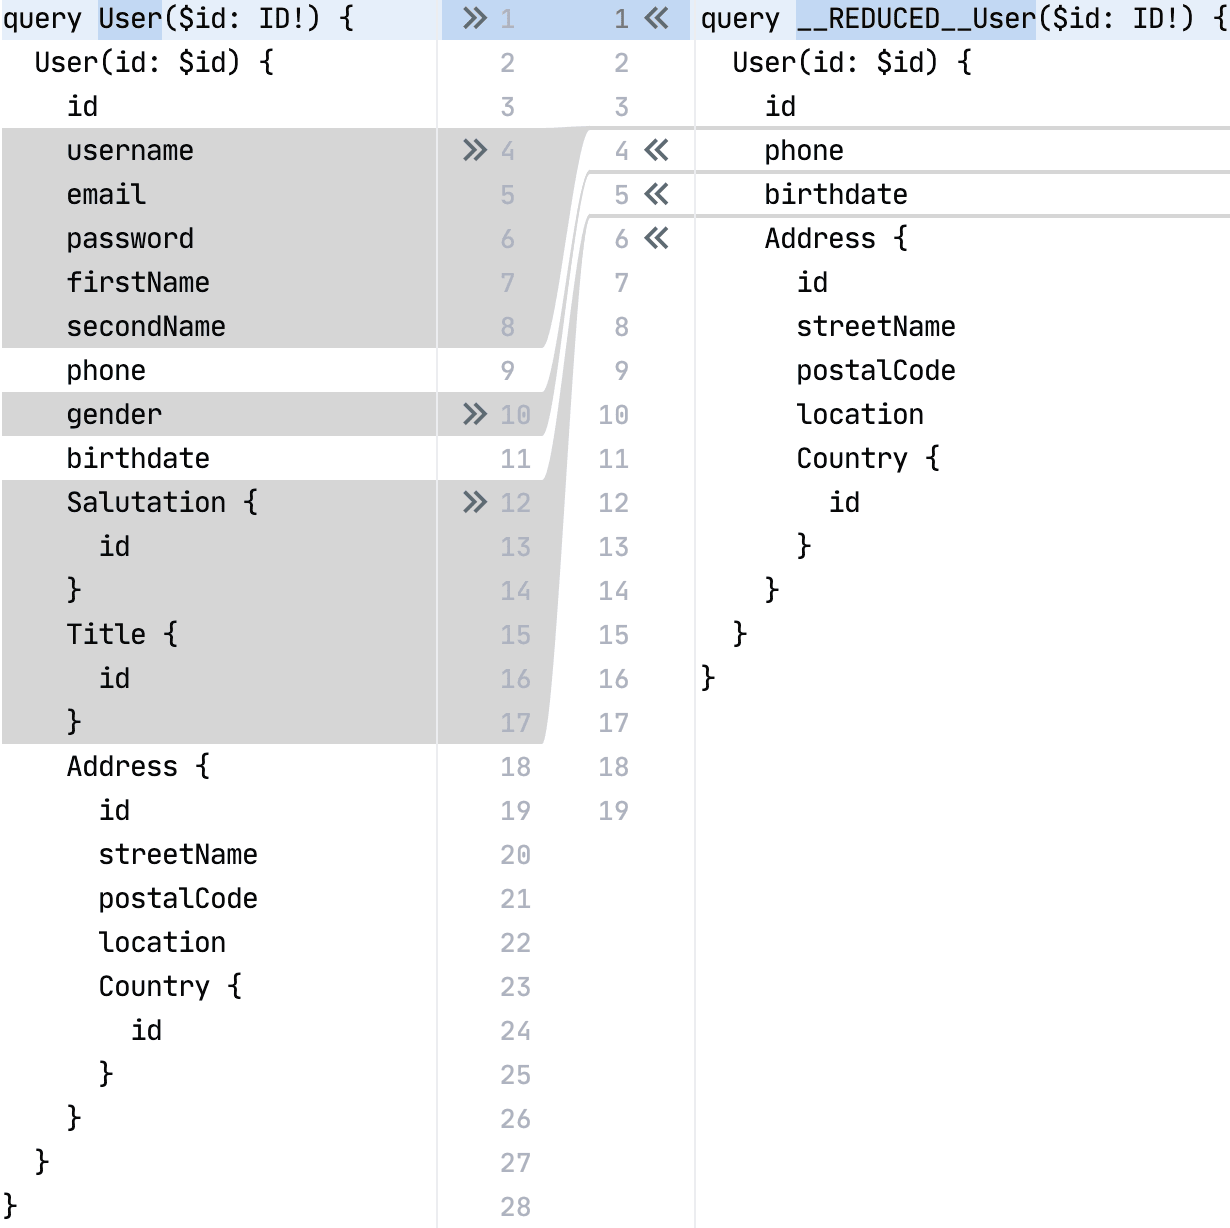
\includegraphics[width=0.6\linewidth]{images/reduction-graphql-examples/compare-user-reduced-user.png}
  \caption{Comparison of the original user- and reduced user-query.}\label{fig:applied-methods:comparison-user-reduced-user}
  \end{figure}
\fi

\subsection{Comparison between queries and reduced queries}

This section shows the difference in request- and response-size of different queries. The table \ref{table:code:comparison-user-reduction} shows the difference in size of the user-detail query, with the query reduction that was explained in the previous section. By removing 8 fields from the request, the size of the requests were reduced by 30\ or by 161 bytes. When querying 10 users a total of 1.61 KB can be saved. The response-size is reduced by 42\ on average. 2.55 KB in response-size is saved if 10 users are queried.

\ifshowTables
\begin{table}[H]
  \begin{tabular}{|l|l|l|l|l|}
  \hline
  Query & Request Diff (\%) & Request Diff (B) & Response Diff (\%) & Response Diff (B) \\
  \hline
  User & 30\ & 161 & 42\ & 257 \\
  \hline
  User & 30\ & 161 & 42\ & 257 \\
  \hline
  User & 30\ & 161 & 41\ & 257 \\
  \hline
  User & 30\ & 161 & 42\ & 244 \\
  \hline
  User & 30\ & 161 & 43\ & 251 \\
  \hline
  User & 30\ & 161 & 42\ & 271 \\
  \hline
  User & 30\ & 161 & 42\ & 249 \\
  \hline
  User & 30\ & 161 & 41\ & 263 \\
  \hline
  User & 30\ & 161 & 41\ & 248 \\
  \hline
  User & 30\ & 161 & 41\ & 252 \\
  \hline
  \hline
  \textbf{AVG} & \textbf{30\%} & - & \textbf{42\%} & -  \\
  \hline
  \textbf{SUM} & - & \textbf{1610 (1.61 KB)} & - & \textbf{2549 (2.55 KB)} \\
  \hline
  \multicolumn{5}{l}{16 fields, 8 Fields Removed, 8 remaining}
  \end{tabular}
  \caption{Comparison of the user-detail query in request- and response-sizes.}\label{table:code:comparison-user-reduction}
\end{table}
\fi

The table \ref{table:code:comparison-contract-reduction} shows the difference for the contract-detail query. By running the list-query for all contracts 10 fields from the 17 can be removed from the query. Therefore only 7 from the 17 fields are remaining inside the query. The requests can be reduced by an average of 38\ or by 207 bytes. When using the application and querying 10 detail-views of the contract 2.07 KB can be saved. The size of the response from the GraphQL backend can be reduced by about 58\. 3.96 KB in response-size is saved if 10 contracts are queried.

 \ifshowTables
 \begin{table}[H]
   \begin{tabular}{|l|l|l|l|l|}
   \hline
   Query  & Request Diff (\%)  & Request Diff (B) & Response Diff (\%) & Response Diff (B)  \\
   \hline
   Contract & 38\ & 207 & 58\ & 394 \\
   \hline
   Contract & 38\ & 207 & 58\ & 378 \\
   \hline
   Contract & 38\ & 207 & 59\ & 403 \\
   \hline
   Contract & 38\ & 207 & 60\ & 408 \\
   \hline
   Contract & 38\ & 207 & 60\ & 409 \\
   \hline
   Contract & 38\ & 207 & 57\ & 370 \\
   \hline
   Contract & 38\ & 207 & 58\ & 393 \\
   \hline
   Contract & 38\ & 207 & 58\ & 407 \\
   \hline
   Contract & 38\ & 207 & 59\ & 400 \\
   \hline
   Contract & 38\ & 207 & 58\ & 389 \\
   \hline
   \hline
   \textbf{AVG} & \textbf{38\%} & - & \textbf{58\%} & - \\
   \hline
   \textbf{SUM} & - & \textbf{2070 (2.07 KB)} & - & \textbf{3951 (3.95 KB)} \\
   \hline
   \multicolumn{5}{l}{17 fields, 10 Fields Removed, 7 remaining}
   \end{tabular}
   \caption{Comparison of the contract-detail query in request- and response-sizes}\label{table:code:comparison-contract-reduction}
 \end{table}
 \fi
